\section{Transformada Rápida de Fourier}

\begin{frame}[fragile]{DFT em $O(N\log N)$}

    \begin{itemize}
        \item A divisão e conquista pode ser aplicada no cálculo da DFT para reduzir sua
            complexidade assintótica

        \item Na etapa de divisão o sinal é dividido em duas partes de tamanhos aproximadamente
            iguais

        \item A conquista acontece quando o sinal tem uma única amostra: neste caso a transformada
            discreta coincide com a própria amostra

        \item A fusão permite o cálculo da DFT do sinal a partir das DFTs das duas partes

        \item Se a fusão for feita em $O(N)$, a recorrência se torna
        \[
            f(N) = 2f(N/2) + (N)
        \]

        \item O Teorema Mestre nos diz que a complexidade da transformada passa a ser $O(N\log N)$

        \item Esta versão da DFT é denominada \textit{Fast Fourier Transform} (FFT)
    \end{itemize}

\end{frame}

\begin{frame}[fragile]{Decomposição do sinal FFT}

    \begin{itemize}
        \item Considere o sinal $(a_k) = a_0, a_1, \ldots, a_{N-1}$

        \item Assuma, sem perda de generalidade, que $N = 2^t$, para algum $t$ natural

        \item Se $N$ não for uma potência de dois, basta adicionar um número suficiente de amostras
            $a_i = 0$ ao sinal até que $N$ se torne uma potência de dois

        \item A etapa de divisão, também denominada decomposição do sinal, o sinal é separado
            em duas partes de tamanho $N/2$: as amostras cujos índices são pares $(e_k)$ e as 
            amostras cujos índices são ímpares $(o_k)$

        \item Assim,
        \[
            (e_k) = a_0, a_2, a_4, \ldots, a_{N - 2}
        \]
        e
        \[
            (o_k) = a_1, a_3, a_5, \ldots, a_{N - 1}
        \]
    \end{itemize}

\end{frame}

\begin{frame}[fragile]{Visualização da decomposição do sinal}

    \begin{figure}
        \centering

        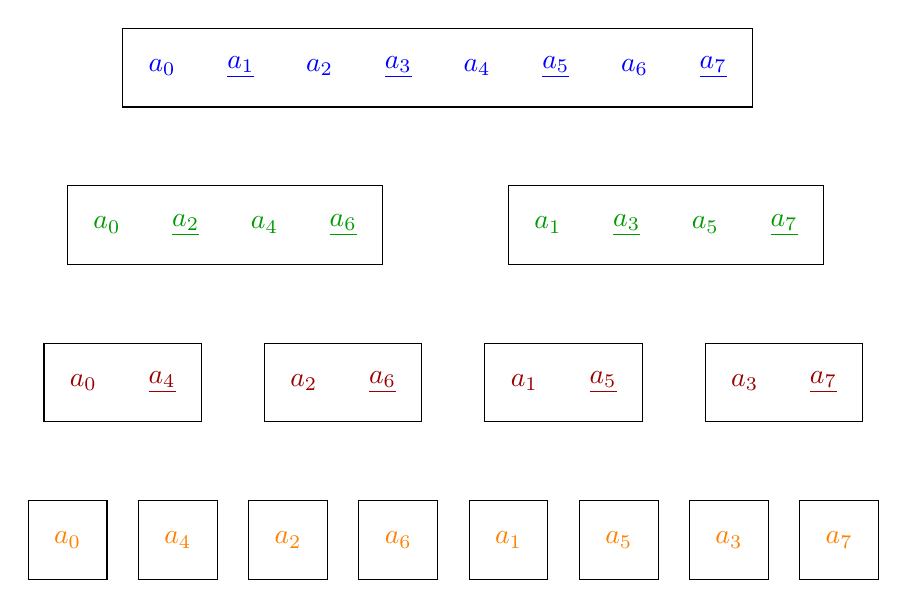
\begin{tikzpicture}

           \draw (1.2, 6) rectangle (9.2, 7);

           \foreach \x in {1,...,4}
           {
                \pgfmathtruncatemacro{\label}{2*\x - 2};
                \node at (2*\x - 1 + 0.7, 6.5) { \textcolor{blue}{{$a_{\label}$}} };
           }

           \foreach \x in {1,...,4}
           {
                \pgfmathtruncatemacro{\label}{2*\x - 1};
                \node at (2*\x + 0.7, 6.5) { \textcolor{blue}{\underline{$a_{\label}$}} };
           }

           \foreach \x in {0,...,1}
                \draw (4*\x + 0.4*4*\x + 0.5, 4) rectangle (4*\x + 0.4*4*\x + 4.5, 5);

           \foreach \x in {0,...,1}
           {
                \pgfmathtruncatemacro{\label}{4*\x};
                \node at (2*\x + 1, 4.5) { \textcolor{green!60!black}{{$a_{\label}$}} };
           }

           \foreach \x in {0,...,1}
           {
                \pgfmathtruncatemacro{\label}{4*\x + 2};
                \node at (2*\x + 2, 4.5) { \textcolor{green!60!black}{\underline{$a_{\label}$}} };
           }

           \foreach \x in {0,...,1}
           {
                \pgfmathtruncatemacro{\label}{4*\x + 1};
                \node at (2*\x + 6.6, 4.5) { \textcolor{green!60!black}{{$a_{\label}$}} };
           }

           \foreach \x in {0,...,1}
           {
                \pgfmathtruncatemacro{\label}{4*\x + 3};
                \node at (2*\x + 7.6, 4.5) { \textcolor{green!60!black}{\underline{$a_{\label}$}} };
           }

           \node at (0.7, 2.5) { \textcolor{red!60!black}{$a_0$} };
           \node at (1.7, 2.5) { \textcolor{red!60!black}{\underline{$a_4$}} };
 
           \node at (3.5, 2.5) { \textcolor{red!60!black}{$a_2$} };
           \node at (4.5, 2.5) { \textcolor{red!60!black}{\underline{$a_6$}} };

           \node at (6.3, 2.5) { \textcolor{red!60!black}{$a_1$} };
           \node at (7.3, 2.5) { \textcolor{red!60!black}{\underline{$a_5$}} };

           \node at (9.1, 2.5) { \textcolor{red!60!black}{$a_3$} };
           \node at (10.1, 2.5) { \textcolor{red!60!black}{\underline{$a_7$}} };

           \foreach \x in {0,...,3}
                \draw (2*\x + 0.4*2*\x + 0.2, 2) rectangle (2*\x + 0.4*2*\x + 2.2, 3);

            \foreach \x in {0,...,7}
                \draw (\x + 0.4*\x, 0) rectangle (\x + 0.4*\x + 1, 1);

           \node at (0.5, 0.5) { \textcolor{orange}{$a_0$} };
           \node at (1.9, 0.5) { \textcolor{orange}{$a_4$} };
           \node at (3.3, 0.5) { \textcolor{orange}{$a_2$} };
           \node at (4.7, 0.5) { \textcolor{orange}{$a_6$} };
           \node at (6.1, 0.5) { \textcolor{orange}{$a_1$} };
           \node at (7.5, 0.5) { \textcolor{orange}{$a_5$} };
           \node at (8.9, 0.5) { \textcolor{orange}{$a_3$} };
           \node at (10.3, 0.5) { \textcolor{orange}{$a_7$} };

        \end{tikzpicture}

    \end{figure}

\end{frame}


\begin{frame}[fragile]{Decomposição $\times$ ordenação}

    \begin{itemize}
        \item Gerando a decomposição por meio da alocação de novos dois subvetores com as cópias
            dos elementos de índices pares e ímpares permite uma implementação \textit{top-down}
            da FFT

        \item Para uma implementação \textit{bottom-up}, é preciso entender
            o padrão subjacente que surge desta decomposição

        \item De fato, os elementos que ocupam as folhas nas árvores de decomposição tem índices
            que correspondem à ordenação dos números $\{ 0, 1, 2, \ldots, N - 1\}$ usando como
            critério a inversão de sua representação binária

        \item Assim, por meio de um comparador customizado o este ordenação pode ser feita 
            com complexidade $O(N\log N)$, o que não modifica a complexidade da FFT como um todo
    \end{itemize}

\end{frame}

\begin{frame}[fragile]{Visualização da ordenação por padrão binário invertido}

    \begin{table}
    \centering
    \begin{tabular}{>{\tt}c>{\tt}c>{\tt}c}
        \toprule
        \textbf{Índice} & \textbf{Padrão invertido} & \textbf{Padrão original} \\
        \midrule
            0 & 000 & 000 \\ 
            \rowcolor[gray]{0.9}
            4 & 001 & 100 \\ 
            2 & 010 & 010 \\ 
            \rowcolor[gray]{0.9}
            6 & 011 & 110 \\ 
            1 & 001 & 100 \\ 
            \rowcolor[gray]{0.9}
            5 & 101 & 101 \\ 
            3 & 110 & 011 \\ 
            \rowcolor[gray]{0.9}
            7 & 111 & 111 \\ 
    \end{tabular}
    \end{table}

\end{frame}


\begin{frame}[fragile]{Implementação da ordenação por padrão binário}
    \inputsnippet{cpp}{1}{18}{codes/order.cpp}
\end{frame}

\begin{frame}[fragile]{Implementação da ordenação por padrão binário}
    \inputsnippet{cpp}{19}{39}{codes/order.cpp}
\end{frame}
